\documentclass{ximera}
  \outcome{Calculate limits using the limit laws}
\begin{document}
\begin{problem}

  Two numbers, $x$ and $y$, are shown below on a number line.
  \begin{image}
    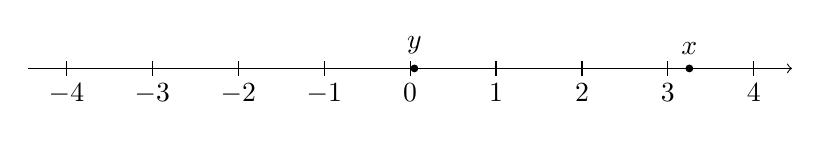
\begin{tikzpicture}[x=0.09\textwidth]
      \draw[-{>[scale=1.75]}] (-0.4\textwidth,0) -- (0.4\textwidth,0);
      \foreach \x in {-4,...,4} {%
        \draw (\x,-.1) -- (\x,.1);
        \node[anchor=north,yshift=-2pt] at (\x,0) {$\x$};
      }
      \draw (3.25,0) node [circle,fill,inner sep=1pt,label=above:$x$](e){};
      \draw (0.05,0) node [circle,fill,inner sep=1pt,label=above:$y$](e){};
    \end{tikzpicture}
  \end{image}
  What can be said about $x/y$?
  \begin{multipleChoice}
    \choice{$x/y$ is very negative.}
    \choice{$x/y$ is close to zero and negative.}
    \choice{$x/y$ is close to zero and positive.}
    \choice[correct]{$x/y$ is large and positive.}
  \end{multipleChoice}
\end{problem}
\end{document}
